\section{Topology Class Reference}
\label{class_topology}\index{Topology@{Topology}}
Inheritance diagram for Topology::\begin{figure}[H]
\begin{center}
\leavevmode
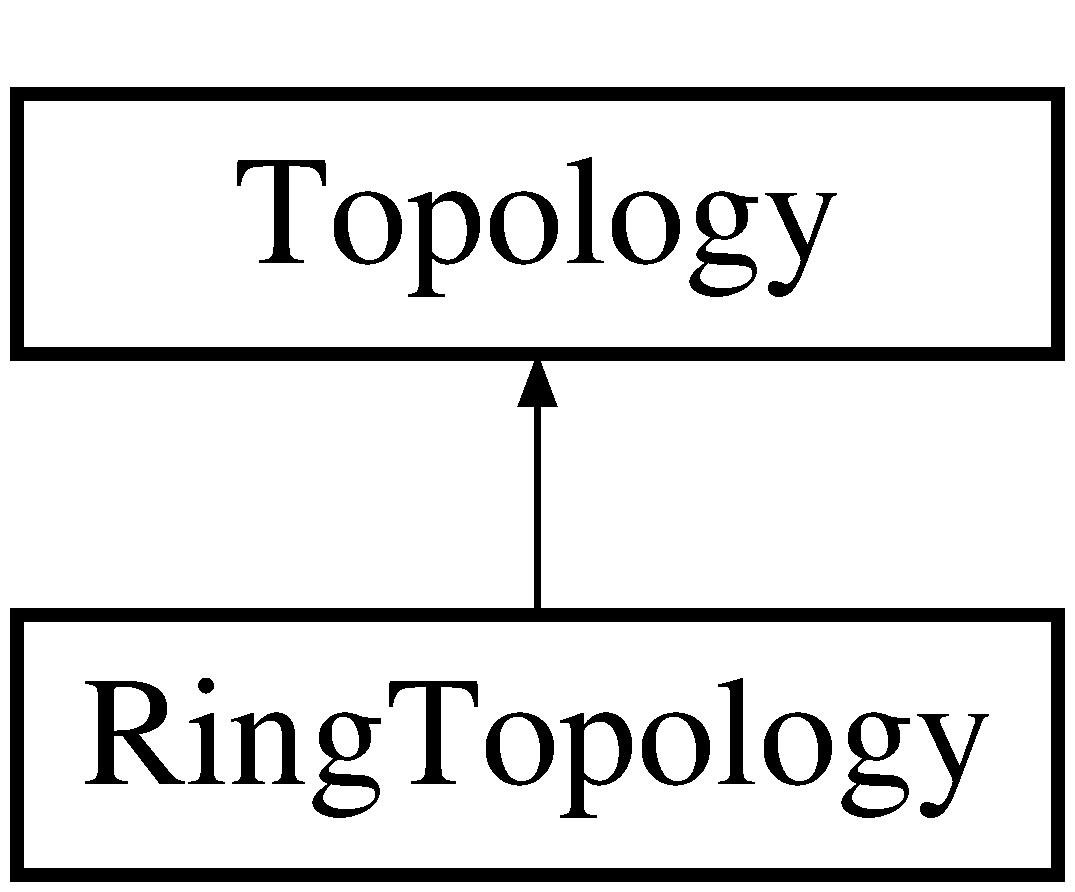
\includegraphics[height=2cm]{class_topology}
\end{center}
\end{figure}
\subsection*{Public Member Functions}
\begin{CompactItemize}
\item 
virtual {\bf $\sim$Topology} ()\label{class_topology_3e447669757c8311c7f6f8edc705abf2}

\item 
void {\bf add} ({\bf Cooperative} \&\_\-\_\-mig)\label{class_topology_62bc46d8c20fdc71dad9e7c7a0d7aded}

\item 
virtual void {\bf set\-Neighbors} ({\bf Cooperative} $\ast$\_\-\_\-mig, std::vector$<$ {\bf Cooperative} $\ast$ $>$ \&\_\-\_\-from, std::vector$<$ {\bf Cooperative} $\ast$ $>$ \&\_\-\_\-to)=0\label{class_topology_86c006ad698649b2ba5016a5ddd619ce}

\end{CompactItemize}
\subsection*{Protected Attributes}
\begin{CompactItemize}
\item 
std::vector$<$ {\bf Cooperative} $\ast$ $>$ {\bf mig}\label{class_topology_247a2faa8568b678f0b7b11e62c7812c}

\end{CompactItemize}


\subsection{Detailed Description}




Definition at line 31 of file topology.h.

The documentation for this class was generated from the following files:\begin{CompactItemize}
\item 
topology.h\item 
topology.cpp\end{CompactItemize}
